% This is samplepaper.tex, a sample chapter demonstrating the
% LLNCS macro package for Springer Computer Science proceedings;
% Version 2.20 of 2017/10/04
%
\documentclass[runningheads]{llncs}
\usepackage{listings}
%
\usepackage{graphicx}
% Used for displaying a sample figure. If possible, figure files should
% be included in EPS format.
%
% If you use the hyperref package, please uncomment the following line
% to display URLs in blue roman font according to Springer's eBook style:
% \renewcommand\UrlFont{\color{blue}\rmfamily}

\usepackage{german}
\usepackage[utf8]{inputenc}

\begin{document}
%
\title{SmartShop}
%
%\titlerunning{Abbreviated paper title}
% If the paper title is too long for the running head, you can set
% an abbreviated paper title here
%
\author{Alexander Brockmann}
%
% First names are abbreviated in the running head.
% If there are more than two authors, 'et al.' is used.
%
\institute{7202423\\
\email{{alexander.brockmann002}@stud.fh-dortmund.de}}


%
\maketitle              % typeset the header of the contribution

\section{Beschreibung der Projektidee}
Durch Covid-19 ist es in vielen Bereichen des täglichen Lebens aufgefallen, wie wichtig es ist, Menschen zu koordinieren beziehungsweise große Menschenansammlungen zu vermeiden.
Auch außerhalb von Pandemien lässt sich die bestehende Infrastruktur durch eine gleichmäßige Verteilung bestmöglich nutzen.
Auf diesen Erkenntnissen basierend entstand die Idee einer verteilten Anwendung zur Optimierung der Auslastung von Supermärkten.

Die Anwendung soll dem Anwender Informationen zur aktuellen Auslastung eines Supermarktes geben.
Außerdem sollen dem Anwender Supermärkte anhand der Auslastung und der Erreichbarkeit empfohlen werden.
Zu dem System gehören die Ein- und Ausgangssensoren von Supermärkten, Standortdaten von Nutzern, eine SmartAI zum prognostizieren von möglichen Auslastungen, eine Datenbank zum Vorhalten von sensorischen Daten, ein Frontend Client zur Bedienung durch den Nutzer und ein Backend zum Aufbereiten und Bereitstellen der Daten.

Durch die Kombination von statistischen Erfahrungswerten mit Umweltdaten wie dem Wetter, stattfindenden Events oder Baustellen und Streckensperrungen soll bestimmt werden, wann welcher Supermarkt am besten zu nutzen ist.
Darüber hinaus sollen Empfehlungen zur Route beziehungsweise den zu nutzenden öffentlichen Verkehrsmitteln gegeben werden.

Zur Anwendungsdomäne gehören folgende Entitäten:

\begin{description}
	\item[Sensordaten] Ein Sensor erfasst seinen aktuellen Standort, die aktuelle Zeit und die Anzahl an Kunden in seinem zugewiesenen Bereich. Ein solcher Sensor ist mittlerweile in vielen Supermärkten im Einsatz. Die oben genannten Attribute werden in der Entität \textit{SensorData} zusammengefasst und in regelmäßigen Abständen bereitgestellt.
	\item[Nutzer] Ein Nutzer hat einen Standort, welcher vom Client bei der Anfrage an das System weitergegeben wird. Zusätzlich wählt der Nutzer aus, nach welcher Art Shop er suchen möchte. Auf dieser Basis bekommt er einen Shop und gegebenenfalls eine Route empfohlen.
	\item[GeoPosition] Die GeoPosition gibt die geografische Position basierend auf dem Längen- und Breitengrad an.
	\item[SensorArea] Eine SensorArea ist ein abstraktes Konstrukt, das jeweils von Sensor und Shop implementiert wird. Er stellt einen Bereich dar der durch einen oder mehr Sensoren abgedeckt werden kann.
	\item[Shop] Der Shop repräsentiert ein Geschäft oder eine Ansammlung von Geschäften, beispielsweise ein Einkaufszentrum. Zu einem Shop gehört jeweils ein Name, ein ShopType, die Größe der Ladenfläche, die Kapazität und die GeoPosition. Zusätzlich wird noch eine Liste an SensorAreas gespeichert.
	\item[ShopType] Der ShopType gibt an, um was für eine Art Shop es sich handelt.
Abhängig von der Art des Shops und seiner Größe wird auch die Kapazität berechnet.
	
\end{description}


\section{Architektur des Projektes}

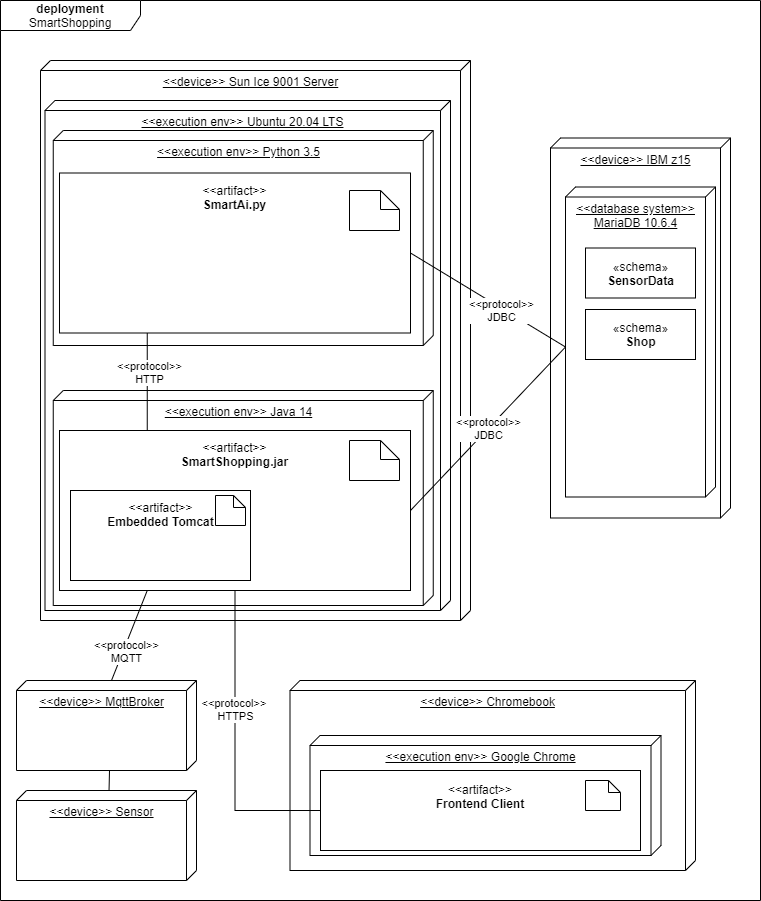
\includegraphics[width=\linewidth]{images/deployment_diagram}


\subsection{Beschreibung der Systemarchitektur}


Der Server, auf dem die Anwendung läuft, kann beispielsweise ein Sun Ice 9001 sein.
Dieser wird mit dem Betriebssystem Ubuntu 20.04 LTS betrieben, da es Open Source, kostenlos und gut dokumentiert ist.
Darin wird zum einen die SmartAi.py ausgeführt, welche in der Laufzeitumgebung Python 3.5 läuft. 
Python ist eine gängige Sprache für KI-Lösungen verwendet wird.
Zum anderen wird dort die SmartShopping.jar in der Laufzeitumgebung Java 14 ausgeführt.
Auf Grund der im Studium gesammelten Erfahrung wurde sich für Java in Kombination mit Spring Boot entschieden.
Die Spring-Applikation stellt den in Spring Boot integrierten Embedded Tomcat bereit.
Die SmartAi.py und die SmartShopping.jar kommunizieren intern via REST-Schnittellen mit dem HTTP-Protokoll.
Mit dem Datenbankserver kommunizieren sie mit dem JDBC-Protokoll.
Der Datenbankserver wird beispielsweise auf einem IBM z15 ausgeliefert.
Auf diesem läuft eine MariaDB 10.6.4.
In der Datenbank gibt es die Schemata SensorData und Shop.

Des Weiteren liefert das Backend den Frontend Client in Form einer Thymeleaf\footnote{\url{https://www.thymeleaf.org/}}-Anwendung aus.
Der Frontend Client wird beispielsweise auf einem Chromebook ausgeliefert und kann dann über einen Browser beispielsweise Chrome aufgerufen werden.
Backend und Frontend kommunizieren über das HTTPS-Protokoll.
Außerdem werden im Verteilungsdiagramm ein MqttBroker und die dazu gehörenden Sensoren dargestellt.
Da der Fokus nicht auf dem Erheben der Daten liegt, wird nicht näher auf den MqttBroker und die dazu gehörenden Sensoren eingegangen.

\subsection{Einordnung der Architekturentscheidungen}
Der Architekturstil nach Starke ist ein heterogenes System, da die Kommunikation zwischen den Services über REST-Schnittstellen realisiert ist (vgl. \cite{starke2015effektive}).
Des Weiteren erfolgt die Kommunikation zwischen Anwendung via HTTP, HTTPS und JDBC.
Die Architektur wurde gewählt, um die Anwendung möglichst modular zu halten und so eine gute Austauschbarkeit von Komponenten zu gewährleisten.

\newpage
\section{Entwurfsmuster}

\subsection{Darstellung der Entwurfsmuster als Klassendiagramm}
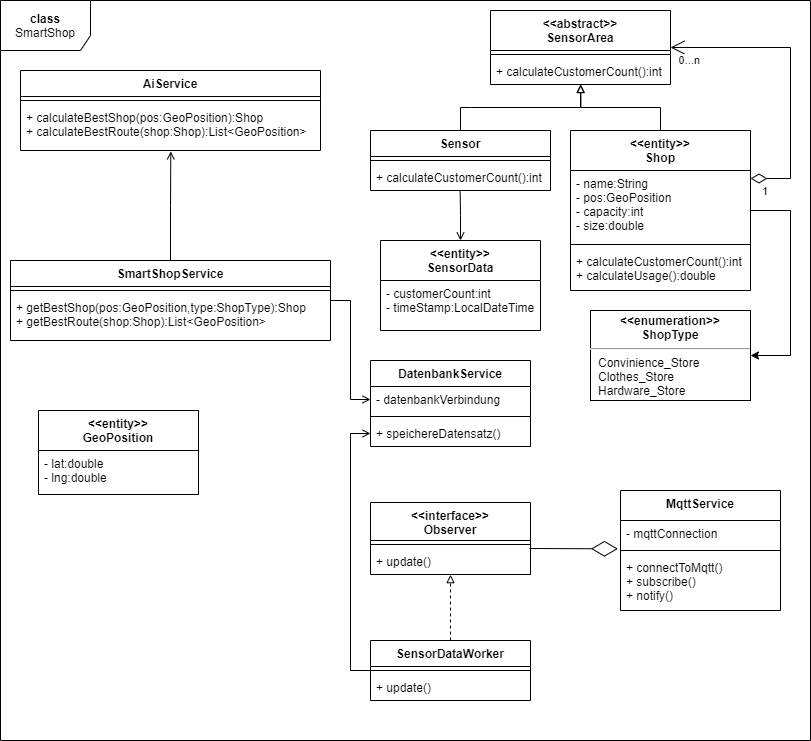
\includegraphics[width=\linewidth]{images/OOD-Klassendiagram}
\begin{description}
\item[Komposit]
Das Komposit wird verwendet, damit komplexe Strukturen wie zum Beispiel Einkaufszentren dargestellt werden können.
Dafür wird die abstrakte Klasse SensorBereich (SensorArea) genutzt. Diese besitzt eine Methode zur Berechnung der Anzahl an Personen in der SensorArea, dazu muss jeweils die Anzahl an Personen in den untergeordneten SendorAreas ermittelt werden.
Eine SensorArea kann dabei ein Sensor oder ein Shop sein.
Handelt es sich um einen Shop, so verfügt dieser zusätzlich über eine Liste untergeordneter SensorAreas.
In einem normalen Supermarkt können diese den verschiedenen Eingängen des Supermarktes zugeordnet sein.
Bei einem Einkaufszentrum beispielsweise können die untergeordneten SensorAreas auch Shops sein.
Dadurch kann die SensorArea beliebig skaliert und die eigentliche Anzahl an Personen in der SensorArea rekursiv berechnet werden.  
Diese Skalierbarkeit ist der Vorteil dieses Entwurfsmusters und wurde deswegen ausgewählt. 
\item[Beobachter-Muster]
Für das Beobachter-Muster wurde zunächst die Klasse MqttService modelliert. 
Diese nimmt Sensordaten vom Mqtt-Sensordaten-Server entgegen.
Damit diese Daten in das richtige Schema der Datenbank persistiert werden können, bietet der Service die Möglichkeit sich darauf zu subscriben.
Eingetragene Observer werden über eingehende Sensordaten informiert.
Für die Observer wird ein Interface bereit gestellt.
Diese Schnittstelle wird von einer konkreten Klasse implementiert, dem SensorDataWorker.
Dieser SensorDataWorker filtert die Daten, ruft den DatenbankService auf und übergibt die zu speichernden Daten.
Durch dieses Beobachter-Muster ist es möglich, weitere Daten über separate Beobachter zu verarbeiten, ohne das bisherige Beobachter angepasst werden müssen.
\end{description}


\subsection{Begründung}
In diesem Kontext wurde das Kompositum-Muster gewählt, da es für die Darstellung der Beziehung zwischen SensorArea, Sensor und Shop geeignet ist.
Dabei entspricht SensorArea der Komponente, Sensor einem Blatt und Shop dem Kompositum.
Der Vorteil des Kompositum-Musters ist, dass die SensorArea beliebig erweitert werden kann und es dabei zweitrangig ist, um welche Attribute und Methoden die Shops beziehungsweise andere Komponenten erweitert werden. 
Ein weiterer Vorteil des Kompositum-Musters ist die variable Tiefe, da sich so auch komplexe Einkaufszentren mit verschachtelten Shops abbilden lassen.
Dies ist allerdings auch ein Nachteil, da es zu einer unübersichtlichen Datenstruktur kommen kann.

Das Beobachter-Muster wurde gewählt, da es eingehende Signale von den Sensoren beziehungsweise Sensornachrichten automatisch verarbeitet und speichert.
Dieses Muster könnte durch das Zustands-Muster ausgetauscht werden.
Das Zustands-Muster würde in der konkreten Implementierung ebenfalls auf eingehende Nachrichten warten beziehungsweise reagieren, es könnte beispielsweise als ein Buffer agieren welcher Nachrichten sammelt und erst auf Anfrage Daten weiterleitet oder speichert.
Dadurch ist allerdings der Server für das stetige Abfragen der Daten verantwortlich.
Dieses sogenannte Busy Waiting ist sehr ressourcenintensiv und sollte daher vermieden werden (vgl. \cite{RJ2021}).

\newpage
\section{Beschreibung der Kernfunktionalität}
Eine der Kernfunktionalitäten der verteilten Anwendung ist es, die Auslastung von Shops zu ermitteln und mit diesen Informationen weiter zu arbeiten.
Daher stellen wir in diesem Abschnitt die Funktionalität zur Ermittlung der Auslastung eines Shops vom Typ ShoppingCenter dar.

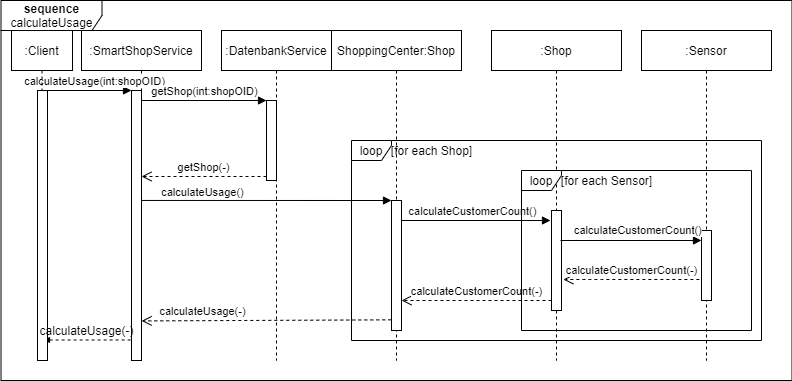
\includegraphics[width=\linewidth]{images/Sequenzdiagramm}
In dem im Sequenzdiagramm beschriebenen Beispiel möchte ein Client die Auslastung eines bestimmten Shops abfragen und ruft daher die Methode calculateUsage auf dem SmartShopService auf.
\\

\textbf{SmartShopService}: In diesem Beispiel wird davon ausgegangen, dass es bei der Auflösung einer bestimmten ShopOID nicht zu einem Fehler kommt sondern die Auflösung immer erfolgreich ist.
Die Methode \textbf{\textit{calculateUsage}} berechnet die aktuelle Auslastung des Shops, welcher über seine ShopOID angefordert wird.
\begin{lstlisting}[language=Java, basicstyle=\scriptsize]
public int calculateUsage(int shopOID){
	Shop shop = datenbankService.getShop(shopOID);
	return shop.calculateUsage();
}
\end{lstlisting}


\textbf{DatenbankService}: Beim Aufruf der Datenbank wird davon ausgegangen, dass es zu keinem Fehler kommt und die Datenbank den Shop mittels Primärschlüssel findet.
Die genaue Anfrage an die Datenbank wird durch die Funktion \textbf{\textit{getShopByPrimaryKey}} abstrahiert.
\begin{lstlisting}[language=Java, basicstyle=\scriptsize]
public Shop getShop(int shopOID){
	return getShopByPrimaryKey(shopOID);
}
\end{lstlisting}

\break
\textbf{Shop}: Zur Berechnung der Anzahl an Personen in der Methode \textbf{\textit{calculateCustomerCount}} des Shops wird über die Liste der SensorAreas iteriert.
Für jede SensorArea wird die wiederum die Anzahl an Personen berechnet und die Rückgabewerte werden im Shop aufsummiert.
Die Methode liefert die aufsummierte Anzahl an Kunden in dem Shop zurück.
\begin{lstlisting}[language=Java, basicstyle=\scriptsize]
public int calculateCustomerCount(){
	int customerCount = 0;
	for (SensorArea sensorArea : this.getSensorAreas()) {
		customerCount += sensorArea.calculateCustomerCount();
	}
	return customerCount;
}
\end{lstlisting}

Die Methode \textbf{\textit{calculateUsage}}, berechnet die momentane Auslastung eines Shops basierend auf seiner Kapazität, der aktuellen Anzahl seiner Kunden und der Anzahl von Kunden seiner untergeordneten SensorAreas.
\begin{lstlisting}[language=Java, basicstyle=\scriptsize]
public int calculateUsage(){
	return this.calculateCustomerCount() / this.capacity;
}
\end{lstlisting}

\newpage
\section{Persistente Datenhaltung}

\subsection{Persistierungansatz}
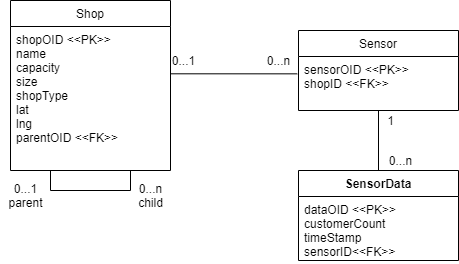
\includegraphics[width=\linewidth]{images/Datamodel}
\begin{description}
	\item[Shop] Der Shop besitzt eine eindeutige ID, welche als Primärschlüssel dient. 
	Des Weiteren besitzt er folgende Attribute: 
	\begin{description}
		\item [name:] Das Attribut name repräsentiert den Namen des Shops.
		\item [capacity:] Das Attribut capacity speichert die maximale Anzahl an Kunden, die sich in dem Shop aufhalten dürfen.
		\item [size:] Das Attribut size beschreibt die Grundfläche des Shops.
		\item [shopType:] ShopType repräsentiert den Typ des Shops.
		\item [lat, lng:] lat und lng beschreiben den Breiten- und Längengrad des Shops. Die Daten kommen aus der Entität \textbf{GeoPosition}, welche aber in diesem Kontext innerhalb des Shops persistiert wird, da Shop und GeoPosition in einer eins-zu-eins-Beziehung stehen.
		\item [parentOID:] Die parentOID ist ein Fremdschlüssel auf eine möglicherweise übergeordneten SensorArea, das Attribut kann leer sein.
	\end{description} 
	Die Parent-Child-Beziehung beschreibt das im Entwurfsmuster dargestellte Komposit.
	\item[Sensor] Der Sensor besitzt das Feld sensorOID, welches eine eindeutige ID ist und als Primärschlüssel fungiert. Außerdem besitzt er das Attribut shopOID als Fremdschlüssel, welches auf einen Shop verweist, das Attribut kann leer sein.
	\item[SensorData] SensorData besitzt folgende Attribute:
	\begin{description}
		\item[dataOID:] Die dataOID ist eine eindeutige ID und fungiert als Primärschlüssel.
		\item[customerCount:] Das Attribut customerCount repräsentiert die Anzahl an Kunden innerhalb der zugeordneten SensorArea zu dem Zeitpunkt des Erstellens des SensorData-Objektes.
		\item[timeStamp:] Dieses Attribut speichert den Zeitpunkt, zu dem das SensorData-Objekt erstellt wurde.
		\item[sensorOID] SensorOID enthält einen Fremdschlüssel, welcher den zu SensorData gehörenden Sensor identifiziert.
	\end{description}
\end{description}

In der Datenhaltung werden die Entitäten Shop, Sensor und SensorData gespeichert.
Eine weitere Entität wäre die geografische Position, da diese aber in einer eins-zu-eins-Beziehung zur Entität Shop steht, werden die Daten direkt im Shop gespeichert.

Der DatenbankService verwendet Spring Data JPA.
Dadurch werden sowohl die benötigten Tabellen als auch die via Methodennamen definierten Datenbankabfragen automatisch generiert.
Die gewählte Datenbank ist eine MariaDB, welche auf einem eigenen Server ausgeliefert wird.


\subsection{Begründung}
Da die Daten einfach strukturiert sind und eine eindeutige ID besitzen, habe ich mich für eine SQL Datenbank entschieden.
Durch diese Datenstruktur ist ein schneller, sicherer und einfacher Zugriff möglich.
Die gewählte Datenbank ist eine MariaDB, da diese frei verfügbare OpenSource-Lösung zu MySQL ist.
Die Datenbank wird auf einem eigens dafür vorgesehenen Server aufgesetzt, um eine lose Koppelung zu gewährleisten. 
Außerdem können Anwendungen, anders als bei einer In-Memory Datenbank, unabhängig voneinander auf die Datenbank zugreifen.
Ich habe mich für Spring Data JPA entschieden, da es durch Spring standardisiert ist und datenbankunabhängig funktioniert.
Außerdem nimmt es dem Programmierer einiges an Arbeit ab.
Beispielsweise ist es nicht mehr notwendig eigene Abfragen zu definieren, da diese anhand der Methodennamen im entsprechenden Reopsitory Interface generiert werden.
Darüber hinaus werden die Tabellendefinitionen aus den Klassen generiert, sodass es nicht nötig ist, diese manuell zu erstellen.
Auch das Mapping von Fremdschlüsselbeziehungen auf die jeweiligen Objekt geschieht automatisch.
Diese Vorteile überwiegen den Nachteil, dass weitere Abhängigkeiten in den Code geladen werden.

Eine Alternative zu MariaDB wäre neben dem bereits erwähnten MySQL eine dokumentenorientierte Datenbank.
Ich habe mich gegen diese Form von Datenbanken entschieden, da ich mit einem festen Schema arbeiten möchte und NoSQL dies nicht bietet.
Da die Sensordaten mit einem Zeitstempel versehen werden, könnten sie in einer Zeitreihen-Datenbank gespeichert werden.
Hier wird allerdings die MariaDB verwendet damit das Mapping der Fremdschlüssel durch Spring Data JPA abgewickelt wird.

Graphdatenbanken eignen sich für diesen Anwendungsfall nicht, da die zu speichernden Daten nicht in einem Graph dargestellt werden können.
\newpage

\section{Kommunikation}

\subsection{Kommunikationsansatz}
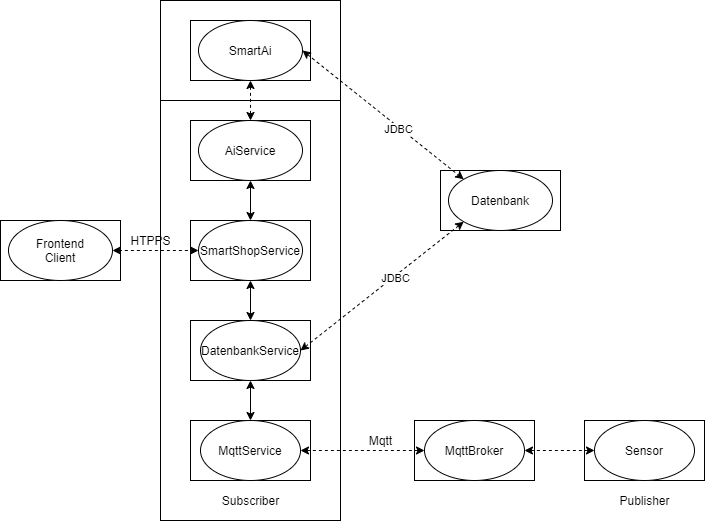
\includegraphics[width=\linewidth]{images/Kommunikation}

Die Kommunikation zwischen SmartAI und dem AiService erfolgt über REST-Schnittstellen mit dem HTTP-Protokoll, diese Kommunikation ist synchron.

Die SmartAi kommuniziert mit dem Datenbankserver via JDBC, diese Kommunikation ist ebenfalls synchron. JDBC ist eine Middleware, welche ein standartisiertes Interface für SQL Datenbanken bereitstellt.

Der Frontend Client kommuniziert mit dem SmartShopService über HTTPS und eine REST-Schnittstelle. Die Kommunikation ist synchron.

Der DatenbankService kommuniziert ähnlich wie die SmartAi über JDBC mit der Datenbank. Die Kommunikation ist synchron mit JDBC als Middleware.

Der MqttService funktioniert nach dem Publish-Subscribe-Prinzip. Der MqttService subscribed sich auf die Nachrichten vom MqttBroker, welcher wiederum die Nachrichten der Sensoren sammelt und an seine Subscriber weiterleitet.
Der MqttBroker dient als Middleware, es wird das MQTT-Protokoll verwendet und die Kommunikation ist asynchron. \\

Die nach außen bereitgestellten Schnittstellen sind vom Backend ausgehend REST-Schnittstellen, um Metainformationen anzufordern, wie zum Beispiel die aktuelle Auslastung eines Shops.
Außerdem gibt es eine Schnittstelle die den besten Weg basierend auf dem aktuellen Standort und dem ausgewählten ShopType zurückgibt.
Beide Daten werden bei der Anfrage als Parameter mitgegeben.
Diese Schnittstellen werden im Regelfall vom Frontend angesprochen.

Außerdem stellt der Datenbankserver eine Schnittstelle bereit, um via SQL Daten anzufordern und zu speichern.
Dieser Endpunkt wird allerdings nur vom Backend über JDBC angesprochen und sollte von außen nicht erreichbar sein.

\subsection{Begründung}
Eine REST API wird in diesem Kontext verwendet, da sie eine einfache und standardisierte Kommunikation zwischen Services in einem verteilten System ermöglicht.
Dadurch ist gewährleistet, dass weitere Services einfach ergänzt und ersetzt beziehungsweise bestehende Services erweitert werden können, ohne dass die Schnittstelle selbst angepasst werden müssen.
Außerdem bietet REST die Möglichkeit Services einfach nach außen, beispielsweise ins World Wide Web, verfügbar zu machen.
Eine Alternative zu REST wären beispielsweise WebSockets\footnote{\url{https://developer.mozilla.org/de/docs/Web/API/WebSockets\_API}}, welche als Basis für einen MessageBroker ähnlich wie bei MQTT verwendet werden können.
In diesem Kontext wurde sich gegen WebSocket entschieden, da die Kommunikation zwischen Client und Server synchron erfolgen kann.
Außerdem würden WebSockets eine nicht benötigte Komplexität in das Projekt bringen.

JDBC wird verwendet, da es als Middleware ein standardisiertes Interface bietet und somit der Programmierer einfach mit dem Datenbankserver kommunizieren kann.
Ähnlich wie bei REST kann auch hier eine direkte Kommunikation verwendet werden, es muss dann allerdings auch der Aufwand betreiben werden und bei Änderungen die Kommunikation anpassen.
Darüber hinaus muss im Datenbankserver eine andere Protokollform aktiviert werden, über die dann kommuniziert werden kann.

Der MqttBroker wird in diesem Kontext verwendet, da er die Kommunikation mit den Sensoren vereinfacht.
So muss der Programmierer sich nicht darum kümmern, wie viele Sensoren existieren und muss nur eingehende Änderungen verarbeiten.
Außerdem werden Änderungen in den Sensordaten so automatisch an den Server gesendet und der Server muss diese Änderungen nicht aktiv abfragen.
So wird Busy Waiting vermieden.
Hier wieder das Problem, man muss über eine Middleware arbeiten, welche nicht zwangsläufig optimiert funktioniert.


\newpage
\bibliographystyle{alphadin}
\bibliography{lit}


\end{document}
